\localeDE{\part{Tutorials: Der schnelle Einstieg}}

\localeDE{
Dieser Teil der Dokumentation soll dem schnellen Einstieg in die Anwendung von \thepackage\ ermöglichen. Er ist in die wichtigsten Anwendungsfälle aufgeteilt und behandelt jeweils die zentralen Aspekte. Es werden jedoch nicht alle Funktionen von \thepackage\ thematisiert. Es soll ein möglichst einfacher Einstieg ermöglicht werden, grundlegende \LaTeX-Fähigkeiten werden jedoch vorausgesetzt.

Die einzelnen Abschnitte behandeln die jeweiligen Themen nur oberflächlich, wobei am Ende der Abschnitte verwandte Makros und Optionen aufgelistet sind, die zum vertiefenden Verständnis beitragen können. Eine detaillierte Dokumentation der zugehörigen Optionen und Makros bietet Teil~\ref{sec:doc}.
}

\localeDE{
  \section{Das erste Arbeitsblatt}
  \label{sec:tut:arbeitsblatt}
}

\localeDE{
Im ersten Abschnitt beschäftigen wir uns mit dem schulischen Tagesgeschäft: der Erstellung eines Arbeitsblattes. 
}

\localeDE{\subsection{Laden der Dokumentenklasse}}

\localeDE{
Der erste Schritt besteht im Laden der Dokumentenklasse. Dies geschieht im einfachsten Fall durch die Zeile
}

\startcode{de}
\begin{codefilecontent*}{doc/tut-de-content-documentclass}
\documentclass{edu}
\end{codefilecontent*}
\endcode


\localeDE{\subsection{Optionen verwenden}}

\localeDE{
Viele Einstellungen von \thepackage\ lassen sich konfigurieren. Da in den Tutorials einige Optionen thematisiert werden, betrachten wir an dieser Stelle einige grundlegende Aspekte.

Dies geschieht über sogenannte \emph{Optionen}. Man unterscheidet verschiedene Typen von Optionen: Einigen Optionen kann ein beliebiger Text (\meta{String}, engl. \emph{string} -- \emph{Zeichenkette}) zugeordnet werden. Andere Optionen erwarten eine Maßeinheit (\meta{Dim}, engl. \emph{dimension} -- \emph{Maßangabe}), z.\,B. in \texttt{cm}, \texttt{mm}, \texttt{pt}, \texttt{ex} oder \texttt{em}. Booleschen Optionen (\meta{Bool}, engl. \emph{boolean} -- \emph{boolesch}) hingegen können die \emph{Wahrheitswerte} \texttt{true} (\emph{wahr}) und \texttt{false} (\emph{falsch}) zugeordnet werden. Boolesche Optionen können alternativ auch ohne Wert angegeben werden, was dem Wert \texttt{true} entspricht. So entspricht z.\,B. die Angabe \texttt{showresults} der Angabe \texttt{showresults=true}. Tabelle \ref{tab:option-types} fasst die Optionstypen zusammen.
}

\localeDE{
\begin{table}[h!tb]
  \centering
  \caption{Typen von Optionen.}
  \label{tab:option-types}
  \medskip
  \begin{tabular}{lll}\toprule
    \sffamily Typ & \sffamily Bezeichnung & \sffamily Beispiel \\\midrule
    Text & \meta{String} & \texttt{autor=Max Mustermann} \\
    Maßeinheit & \meta{Dim} & \texttt{listarraysep=0.5cm} \\
    Boolesch & \meta{Bool} & \texttt{twoup=true} oder \texttt{twoup} \\\bottomrule
  \end{tabular}
\end{table}
}

\localeDE{
Alle Optionen lassen sich direkt beim Laden der Dokumentenklasse konfigurieren. So kann man z.\,B. die Standardschriftgröße durch die Option \opt*{fontsize} auf \opt*{12pt} erhöhen:
}

\startcode{de}
\begin{codefilecontent*}{doc/tut-de-content-options-example-1}
\documentclass[fontsize=12pt]{edu}
\end{codefilecontent*}
\endcode

\localeDE{
Möchte man mehrere Optionen verwenden, werden diese jeweils durch ein Komma getrennt. Man sollte sie -- zugunsten der Lesbarkeit -- in einzelne Zeilen schreiben:
}

\startcode{de}
\begin{codefilecontent*}{doc/tut-de-content-options-example-2}
\documentclass[
  fontsize=12pt,
  footer=false
]{edu}
\end{codefilecontent*}
\endcode

\localeDE{
Viele Optionen können außerdem über die Makros \Macro\edusetup und \Macro\eduoption innerhalb der Präambel (d.\,h. vor Begin von \env*{document}) manipuliert werden. \Macro\edusetup dient dem Ändern mehrerer Optionen, wobei die Wertzuweisungen jeweils durch ein Komma getrennt werden müssen. \Macro\eduoption hingegen ermöglicht nur das Setzen einer Option. Die folgenden Verwendungen der Makros sind beispielsweise äquivalent:
}

\startcode{de}
\begin{codefilecontent*}{doc/tut-de-content-options-edusetup-eduoption}
\edusetup{fontsize=12pt, footer=false}

\eduoption{fontsize}{12pt}
\eduoption{footer}{false}
\end{codefilecontent*}
\endcode


\localeDE{\subsection{Metadaten eingeben}}

\localeDE{
Um die Ordnung in den Unterlagen von SchülerInnen \emph{und} LehrerInnen zu unterstützten, sollten wir zuerst die wichtigsten Metadaten (d.\,h. in diesem Fall Daten \emph{über} das Arbeitsblatt, nicht der Inhalt des Blattes selbst) auf dem Blatt platzieren. Viele der hierfür verwendeten Makros sind bereits aus den Standard-Dokumentenklassen bekannt. Doch ein Blick auf Tabelle~\ref{tab:metadaten} beinhaltet auch Makros, welche von \thepackage\ neu zur Verfügung gestellt werden.

\Notice{In Beispielen dieser Dokumentation, welche auf Metadaten zurückgreifen, werden die Angaben aus Tabelle~\ref{tab:metadaten} verwendet.}
}

\localeDE{
\begin{table}[h!tb]
  \centering
  \caption{Metadaten und die zugehörigen Makros (in alphabetischer Reihenfolge).}
  \label{tab:metadaten}
  \medskip
   \begin{tabular}{lll}\toprule
     \sffamily Datum & \sffamily Makro  & \sffamily Beispiel \\\midrule
     Author & \Macro\author & \Macro\author{Horst Schlämmer} \\ 
     Klasse & \Macro\class & \Macro\class{Klasse 10} \\ 
     Datum & \Macro\date & \Macro\date{6.3.2013} \\ 
     E-Mail & \Macro\email & \Macro\email{horst@intern.et} \\ 
     Gebiet & \Macro\field & \Macro\field{Programmierung} \\ 
     Gruppe & \Macro\group & \Macro\group{A} \\ 
     Lizenz & \Macro\license & \Macro\license{Public Domain} \\ 
     Abkürzung & \Macro\short & \Macro\short{AB1} \\ 
     Fach & \Macro\subject & \Macro\subject{Informatik} \\ 
     Untertitel & \Macro\subtitle & \Macro\subtitle{Wir drehen uns im Kreis} \\ 
     Titel & \Macro\title & \Macro\title{Die While-Schleife} \\ 
     Version & \Macro\version & \Macro\version{1.0} \\ \bottomrule
  \end{tabular}
\end{table}
}

\localeDE{
In Abschnitt~\ref{sec:allg:kopfzeile} wurde bereits erörtert, welche Metadaten sinnvollerweise auf einem Arbeitsblatt gesetzt werden sollten. Diese ergänzen wir in der Präambel unseres Arbeitsblattes:
}

\startcode{de}
\begin{codefilecontent*}{doc/tut-de-content-metadata}
\author{Horst Schlaemmer}
\class{Klasse 10}
\date{6.3.2013}
\field{Zuordnungen}
\subject{Informatik}
\title{Die While-Schleife}
\end{codefilecontent*}
\endcode

\localeDE{
Diese Auswahl an Metadaten sollte in jedem Dokument angegeben werden. Weitere Metadaten können wahlweise verwendet werden. Die Makros bewirken, dass die angegebenen Daten sinnvoll im Titel bzw. in Kopf- oder Fußzeile des Dokuments gesetzt werden.

In einigen Fällen benötigen die Metadaten z.\,B. in der Fußzeile mehr Platz, als zur Verfügung steht.  Aus diesem Grund verfügen die Makros zur Angabe der Metadaten zusätzlich über ein optionales Argument. Dieses kann verwendet werden, um eine kürzere Variante der eigentlichen Daten zu wählen, welche dann in Kopf- bzw. Fußzeile verwendet werden. Dies kann z.\,B. bei einem langen Namen hilfreich sein:
}

\startcode{de}
\begin{codefilecontent*}{doc/tut-de-content-author}
\author[I. Hubmueller-Weidenfels]{Ingeborg Hubmueller-Weidenfels}
\end{codefilecontent*}
\endcode

\localeDE{
Verwandte Makros und Optionen:
\vspace{-0.25\baselineskip}
\begin{multicols}{4}\raggedcolumns
\begin{itemize}
	\item \Macro{\printauthor}
	\item \Macro{\printclass}
	\item \Macro{\printdate}
	\item \Macro{\printemail}
	\item \Macro{\printfield}
	\item \Macro{\printgroup}
	\item \Macro{\printlicense}
	\item \Macro{\printshort}
	\item \Macro{\printsubject}
	\item \Macro{\printsubtitle}
	\item \Macro{\printtitle}
	\item \Macro{\printversion}
\end{itemize}
\end{multicols}
}

\localeDE{\subsection{Kopfzeile erzeugen}}

\localeDE{

Nach diesen "`Vorarbeiten"' widmen wir uns nun dem tatsächlichen Inhalt unseres Arbeitsblattes. Zuerst ergänzen wir hierzu die \env*{document}-Umgebung, welche den Dokumentenkörper beinhaltet:
}

\startcode{de}
\begin{codefilecontent*}{doc/tut-de-content-document}
\begin{document}
  % Hier wird der Inhalt des Dokuments ergaenzt.
\end{document}
\end{codefilecontent*}
\endcode

\localeDE{
Zu Beginn der ersten Seite möchte Horst die Kopfzeile\footnote{In Abschnitt~\ref{sec:allg:kopfzeile} wird erläutert, weshalb standardmäßig lediglich die erste Seite mit einer Kopfzeile versehen wird.} erstellen. Dies geschieht  sehr leicht gleich zu Beginn des Dokumentenkörpers durch das Makro \Macro\makeheader:
}

\startcode{de}
\begin{codefilecontent}{doc/tut-de-content-makeheader}
\makeheader
\end{codefilecontent}
\endcode

\localeDE{
Horst kompiliert seinen Quelltext und freut sich über das Ergebnis: Die Kopfzeile wurde erstellt und beinhaltet die angegebenen Metadaten! Und auch die Fußzeile\footnote{Durch die Option \opt{footer} kann die Fußzeile deaktiviert werden.} wurde automatisch durch \thepackage\ erstellt.
}


\localeDE{
Verwandte Makros und Optionen:
\vspace{-0.25\baselineskip}
\begin{multicols}{4}\raggedcolumns
\begin{itemize}
	\item \opt{headerrulewidth}
\end{itemize}
\end{multicols}
}

\localeDE{\subsection{Titel erzeugen}}

\localeDE{
Als Nächstes soll der Titel unseres Dokumentes eingefügt werden. Nachdem wir den Titel bereits mithilfe des Makros \cs{title} eingegeben haben, muss dieser noch erzeugt werden. Dies geschieht durch das Makro \Macro\maketitle.

Die normale Variante \Macro\maketitle erzeugt einen "`ausführlichen"' Titel, der neben Titel und Untertitel noch fast alle weiteren Metadaten des Dokuments beinhaltet. Somit eignet sich \Macro\maketitle tendenziell für umfangreichere Dokumente (Zusammenfassungen u.\,Ä.):
}

\startcode{de}
\begin{codefilecontent}{doc/tut-de-content-maketitle-1}
\maketitle
\end{codefilecontent}
\endcode

\localeDE{
Aus Platzgründen empfiehlt sich bei Arbeitsblättern die Verwendung der Sternvariante \Macro{\maketitle*}. Diese greift lediglich auf Titel (\cs{title}), Untertitel (\cs{subtitle}), Gruppe (\cs{group}) und Abkürzung (\cs{short}) zurück.
}

\startcode{de}
\begin{codefilecontent}{doc/tut-de-content-maketitle-2}
\maketitle*
\end{codefilecontent}
\endcode

\localeDE{
Verwandte Makros und Optionen:
\vspace{-0.25\baselineskip}
\begin{multicols}{4}\raggedcolumns
\begin{itemize}
	\item \opt{authorstyle}
	\item \opt{classstyle}
	\item \opt{datestyle}
	\item \opt{emailstyle}
	\item \opt{fieldstyle}
	\item \opt{groupbg}
	\item \opt{groupfg}
	\item \opt{groupstyle}
	\item \opt{groupstyle}
	\item \opt{licensestyle}
	\item \opt{shortbg}
	\item \opt{shortfg}
	\item \opt{shortstyle}
	\item \opt{subjectstyle}
	\item \opt{timestampstyle}
	\item \opt{titlebg}
	\item \opt{titlefg}
	\item \opt{titleskip}
	\item \opt{titlestyle}
	\item \opt{versionstyle}
\end{itemize}
\end{multicols}
}

\localeDE{
  \subsection{Aufgaben erstellen}
  \label{sec:tut:aufgaben}
}

\localeDE{
Nun ist es Zeit, endlich Aufgaben zu erstellen. Um Überschriften für Aufgaben zu erstellen (\emph{1.~Aufgbabe}, \emph{2.~Augabe}, \dots) steht das Makro \Macro\exe\ (engl. \emph{exercise} -- \emph{Aufgabe}) zur Verfügung. Um die Aufgaben übersichtlich zu strukturieren, empfiehlt es sich, jeder Aufgabe einen kurzen, prägnanten Titel zu vergeben, was durch das notwendige Argument bewerkstelligt wird. Sollte kein Aufgabentitel gewünscht werden, muss das Klammerpaar ohne Inhalt verwendet werden. Aufgaben werden automatisch arabisch nummeriert. Anschließend verfasst man wie gewünscht den Inhalt der Aufgabe:
}

\startcode{de}
\begin{codefilecontent}{doc/tut-de-content-exe}
\exe{Erste Aufgabe}

Lorem ipsum dolor sit amet ...
\end{codefilecontent}
\endcode


\localeDE{
Es besteht die Möglichkeit, als zusätzliche Gliederungsebene \emph{Unteraufgaben} zu erstellen. Wie bei \cs*{section} und \cs*{subsection} bezeichnet man das entsprechende Pendant zu \Macro\exe\ mit \Macro\subexe. Auch die Verwendung geschieht analog. Die Nummerierung hingegen geschieht durch eine zweite Ebene (1.1, 1.2, 1.3, \dots). Auch \Macro\subexe verfügt über ein notwendiges Argument zur Angabe eines Titels für die Aufgabe. Soll kein Titel verwendet werden, die Klammern dennoch angegeben werden.
}

\startcode{de}
\begin{codefilecontent}{doc/tut-de-content-subexe}
\exe{Aufgabe mit Unteraufgaben}

\subexe{Erste Unteraufgabe}
Lorem ipsum dolor sit amet ...

\subexe{Zweite Unteraufgabe}
Lorem ipsum dolor sit amet ...
\end{codefilecontent}
\endcode

\localeDE{
Mit jeder Erstellung einer neuen Aufgabe durch \Macro\exe beginnt die Nummerierung von \Macro\subexe von vorne.

Unteraufgaben eignen sich hauptsächlich bei sehr Umfangreichen Aufgaben.  Es besteht zusätzlich die Möglichkeit, mehrere kurze Aufgaben in einer alphabetisch nummerierten Liste zu setzen, wie man es z.\,B. aus Mathematik-Büchern kennt: \emph{Teilaufgaben} können zum einen als Liste gesetzt werden. Hierzu dient die Umgebung \env{multiexelist}. Sie verhält sich wie die \env*{itemize}-Umgebung, nummeriert die Einträge jedoch alphabetisch.
}

\startcode{de}
\begin{codefilecontent}{doc/tut-de-content-multiexelist-1}
\begin{multiexelist}
  \item Erste Teilaufgabe
  \item Zweite Teilaufgabe
  \item Dritte Teilaufgabe
\end{multiexelist}
\end{codefilecontent}
\endcode

\localeDE{
%Folgt eine Teilaufgabenliste direkt auf eine (Unter-)Aufgabenüberschrift (d.\,h. auf \Macro\exe oder \Macro\subexe), sollte die Sternvariante \env{multiexelist} verwendet werden, da sie einen zusätzlichen Abstand über der Liste einfügt.

Falls gewünscht, kann über ein optionales Argument ein zusätzlicher Abstand zwischen den Einträgen eingefügt werden. Dies kann z.\,B. bei mathematischen Formeln, welche viel vertikalen Platz benötigen, von Nöten sein:
}

\startcode{de}
\begin{codefilecontent}{doc/tut-de-content-multiexelist-2}
\begin{multiexelist}[2ex]
  \item Erste Teilaufgabe
  \item Zweite Teilaufgabe
  \item Dritte Teilaufgabe
\end{multiexelist}
\end{codefilecontent}
\endcode

\localeDE{
Bei sehr kurzen Teilaufgaben kann die Liste horizontal innerhalb einer Zeile (engl. \emph{inline}) gesetzt werden. Hierzu steht die Umgebung \env{multiexelisti} zur Verfügung. Hierbei werden die Teilaufgaben in einer zentrierten Zeile positioniert. Sollen sie stattdessen innerhalb des aktuellen Absatzes im Fließtext erscheinen kann die Sternvariante \env{multiexelisti*} verwendet werden:
}

\startcode{de}
\begin{codefilecontent}{doc/tut-de-content-multiexelisti}
\begin{multiexelisti}
  \item Erste Teilaufgabe
  \item Zweite Teilaufgabe
  \item Dritte Teilaufgabe
\end{multiexelisti}
\end{codefilecontent}
\endcode

\localeDE{
Möchte man mehrere sehr kurze Teilaufgaben verfassen -- was häufig bei Mathematikaufgaben der Fall ist -- kann die Umgebung \env{multiexearray} verwendet werden. Sie ordnet die Teilaufgaben wie in einer Tabelle an. Als notwendiges Argument benötigt sie deshalb die Anzahl der Spalten und wird ansonsten wie eine Tabelle verwendet. Hier ein Beispiel für den dreispaltigen Satz von Teilaufgaben:
}

\startcode{de}
\begin{codefilecontent}{doc/tut-de-content-multiexearray-1}
\begin{multiexearray}{3}
  Erste Teilaufgabe   & Zweite Teilaufgabe  & Dritte Teilaufgabe \\
  Vierte Teilaufgabe  & Fuenfte Teilaufgabe
\end{multiexearray}
\end{codefilecontent}
\endcode

\localeDE{
Es wir deutlich, dass die unterste Zeile nicht komplett "`befüllt"' werden muss. Es existiert zusätzlich eine Sternvariante \env{multiexearray*}. Diese versetzt die Zellen der Tabelle automatisch in den Mathematikmodus:
}

\startcode{de}
\begin{codefilecontent}{doc/tut-de-content-multiexearray-2}
\begin{multiexearray*}{4}
  2x = 3,5  & 3x = 4  & 4x = 5  & 5x = 6 \\
  6x = 7    & 7x = 8
\end{multiexearray*}
\end{codefilecontent}
\endcode

\localeDE{
Insbesondere beim Satz von Mathematikaufgaben kann es vorkommen, dass sich einzelne Zeilen berühren -- vor allem bei Elementen wie Brüchen oder Integralen, welche viel vertikalen Platz benötigen. Deshalb kann man auch bei \env{multiexearray} und \env{multiexearray*} als optionales Argument einen zusätzlichen Zeilenabstand angeben:
}

\startcode{de}
\begin{codefilecontent}{doc/tut-de-content-multiexearray-3}
\begin{multiexearray*}[2ex]{3}
  \frac{1}{2} x = 3  & \frac{2}{3} x = 4  & \frac{3}{4} x = 5 \\ 
  \frac{4}{5} x = 6  & \frac{5}{6} x = 7  & \frac{6}{7} x = 8
\end{multiexearray*}
\end{codefilecontent}
\endcode

\localeDE{
Innerhalb einer (Unter-)Aufgabe können mehrere Umgebungen mit Teilaufgaben verwendet werden. Die Nummerierung beginnt von vorne, sobald eine (Unter-)Aufgabe beginnt. Eine Limitierung ist jedoch zu berücksichtigen: Es können pro (Unter-)Aufgabe maximal 26 Teilaufgaben erstellt werden -- mehr Kleinbuchstaben bietet das deutsche Alphabet nicht (abgesehen von Umlauten und scharfem S).

Zähler können manuell zurückgesetzt werden. Nach dem Aufruf den Makros \Macro\rstexe, \Macro\rstsubexe oder \Macro\rstmultiexe\ (engl. \emph{reset} -- \emph{zurücksetzen}) beginnt die Nummerierung von \Macro\exe, \Macro\subexe bzw. \env{multiexelist}/\env{multiexearray} bei der nächsten Verwendung von vorne.

Außerdem besteht auf allen Ebenen die Möglichkeit, (optionale) Zusatzaufgaben (auch Bonus- oder "`Sternchen"'-Aufgaben) durch einen Stern zu markieren. Hierzu existieren auf (Unter-)Aufgabenebene die Sternvarianten \Macro{\exe*} und \Macro{\subexe*}. Bei Teilaufgaben muss unterschieden werden: In den Listen \env{multiexelist} und \env{multiexelisti} können Zusatzaufgaben durch \Macro{\item*} erzeugt werden. In \env{multiexearray} kann auf das Makro \Macro\bonus zurückgegriffen werden, welches \emph{vor} dem Wechsel zur nächsten Teilaufgabe (also vor \texttt{\&} bzw. \texttt{\textbackslash\textbackslash}) angegeben werden muss:
}

\startcode{de}
\begin{codefilecontent}{doc/tut-de-content-bonus-exercises}
\exe*{Zusatzaufgabe}

\subexe*{Zusatzaufgabe}

\begin{multiexelist}
  \item Teilaufgabe
  \item Teilaufgabe
  \item* Zusatzaufgabe
\end{multiexelist}

\begin{multiexearray}{3}
  Teilaufgabe \bonus  & Zusatzaufgabe  & Teilaufgabe \bonus \\
  Zusatzaufgabe       & Teilaufgabe
\end{multiexearray}
\end{codefilecontent}
\endcode

\localeDE{
Aufgaben können zusätzlich durch optionale Argumente Verrechnungspunkte zugewiesen werden, welche in Klassenarbeiten relevant sind. Dies wird im entsprechenden Abschnitt~\ref{sec:tut:vp} über Klassenarbeiten thematisiert.
}

\localeDE{
Verwandte Makros und Optionen:
\vspace{-0.25\baselineskip}
\begin{multicols}{3}\raggedcolumns
\begin{itemize}
	\item \opt{arrayafterskip}
	\item \opt{arraybeforeskip}
	\item \opt{exeafterskip}
	\item \opt{exebeforeskip}
	\item \opt{exebg}
	\item \opt{exefg}
	\item \opt{exelabel}
	\item \opt{exelabelbg}
	\item \opt{exelabelfg}
	\item \opt{exelabelstyle}
	\item \opt{exenumberbg}
	\item \opt{exenumberfg}
	\item \opt{exenumberseparator}
	\item \opt{exenumberstyle}
	\item \opt{exestyle}
	\item \opt{multiexenumberfg}
	\item \opt{multiexenumberstyle}
	\item \opt{multiexenumberleft}
	\item \opt{multiexenumberright}
	\item \opt{multiexestyle}
	\item \opt{subexeafterskip}
	\item \opt{subexebeforeskip}
	\item \opt{subexebg}
	\item \opt{subexefg}
	\item \opt{subexelabel}
	\item \opt{subexelabelbg}
	\item \opt{subexelabelfg}
	\item \opt{subexelabelstyle}
	\item \opt{subexenumberbg}
	\item \opt{subexenumberfg}
	\item \opt{subexenumberseparator}
	\item \opt{subexenumberstyle}
	\item \opt{subexestyle}
\end{itemize}
\end{multicols}
}

\localeDE{
  \subsection{Fragen: Freie Antworten und Multiple Choice}
  \label{sec:tut:fragen}
}

\localeDE{
Möchte man Wissen durch Aufgaben überprüfen, bieten Fragen an, welche beantwortet werden sollen. \thepackage\ verfügt über umfangreiche Möglichkeiten, Fragen und zugehörige Antwortmöglichkeiten zu erzeugen.

Das Stellen einer Frage geschieht durch das Makro \Macro\quest\ (engl. \emph{question} -- \emph{Frage}). Es erwartet als notwendiges Argument den Fragentext:
}

\startcode{de}
\begin{codefilecontent}{doc/tut-de-content-quest}
\quest{Eine ganz knifflige Frage ...}
\end{codefilecontent}
\endcode

\localeDE{
Nachdem die Frage gestellt wurde, muss Raum für die Antwort gegeben werden. Hierzu gibt es verschiedene Möglichkeiten. Eine Gruppe von Möglichkeiten setzt voraus, dass die Antworten in irgendeiner Art und Weise schriftlich frei verfasst werden müssen. Die erste dieser Alternativen besteht darin, lediglich freien Platz auf dem Blatt zur Verfügung zu stellen (z.\,B. für eine Skizze). Dies kann durch das Makro \Macro\questblank\ (engl. \emph{blank} -- \emph{unbeschrieben}) umgesetzt werden, welchem als optionales Argument die Höhe des Freiraumes übergeben werden kann. Standardmäßig werden \SI{3}{cm} frei gelassen. Die nächste Möglichkeit sind vorgedruckte Linien zum Verfassen eines Antworttextes. Das Makro \Macro\questtext nimmt hierzu als notwendiges Argument die Anzahl der Zeilen entgegen. Optional kann der Abstand zwischen den Linien angegeben werden. Die letzte Makro \Macro\questtextblank kombiniert die beiden bisherigen Makros. Es erzeugt Linien, welche sich jedoch nicht über die gesamte Textbreite erstrecken. Es besteht hierdurch z.\,B. die Möglichkeit, eine Beschreibung oder Erklärung einzufordern, welche durch eine Skizze verdeutlicht werden soll. Durch zwei notwendige Argumente müssen die Linienanzahl und die Breite der Linien angegeben werden. Ein optionales Argument lässt den Abstand der Linien bestimmen. Im folgenden ein Beipiel mit allen Antwortmöglichkeiten: 
}

\startcode{de}
\begin{codefilecontent}{doc/tut-de-content-quest-answers}
\quest{Erste Frage: 2 cm freier Raum zum Antworten}

\questblank[2cm]

\quest{Zweite Frage: 3 Zeilen Text mit jeweils 1cm Abstand}

\questtext[1cm]{3}

\quest{Dritte Frage: 5 Zeilen mit jeweils 0,75 cm Abstand ueber halbe Textbreite}

\questtextblank[0.75cm]{5}{0.5\linewidth}
\end{codefilecontent}
\endcode

\localeDE{
Die zweite Gruppe von Antwortmöglichkeiten betrifft Multiple-Choice-Fragen. Grundsätzlich wird hier -- wie bei Teilaufgaben in Abschnitt~\ref{sec:tut:aufgaben} -- zwischen Aufgabenlisten und Aufgaben, die tabellarisch angeordnet sind, unterschieden. In beiden Fällen besteht wiederum die Möglichkeit, leere Kästchen zum Ankreuzen oder alphabetisch nummerierte Kästchen zu verwenden. Letztere können im Anschluss besser verglichen werden.

Als Listen stehen die Umgebungen \env{questmclist} (leere Kästchen) und \env{questmclistalph} (alphabetisch nummeriert) zur Verfügung. Sie werden wie gewöhnliche Listen verwendet. Durch ein optionales Argument kann ein zusätzlicher Abstand zwischen den Antwortmöglichkeiten  eingefügt werden, was insbesondere bei der Verwendung von hohen Formeln vonnöten sein kann.
}

\startcode{de}
\begin{codefilecontent}{doc/tut-de-content-quest-lists}
\quest{Erste Frage: Multiple Choice mit leeren Kaestchen}

\begin{questmclist}
  \item Antwortmoeglichkeit 1
  \item Antwortmoeglichkeit 2
\end{questmclist}

\quest{Zweite Frage: Multiple Choice mit leeren Kaestchen (erhoehter Abstand)}

\begin{questmclist}[2ex]
  \item Antwortmoeglichkeit 1
  \item Antwortmoeglichkeit 2
\end{questmclist}

\quest{Dritte Frage: Multiple Choice mit alphabetisch nummerierten Kaestchen}

\begin{questmclistalph}
  \item Antwortmoeglichkeit 1
  \item Antwortmoeglichkeit 2
\end{questmclistalph}
\end{codefilecontent}
\endcode

\localeDE{
Die tabellarische Anordnung von Multiple-Choice-Antworten geschieht durch die Umgebungen \env{questmcarray} (leere Kästchen) und \env{questmcarrayalph} (alphabetisch nummeriert). Als notwendiges Argument erwarten beide Umgebungen die Anzahl der Tabellenspalten. Auch hier kann durch ein optionales Argument der Abstand zwischen den Zeilen angegeben werden. Die Sternvarianten der Umgebungen versetzen die Zellen automatisch in den Mathematikmodus.
}

\startcode{de}
\begin{codefilecontent}{doc/tut-de-content-quest-arrays}
\quest{Erste Frage: Multiple Choice mit leeren Kaestchen in 4 Spalten}

\begin{questmcarray}{4}
  Antwort 1  & Antwort 2  & Antwort 3  & Antwort 4 \\ 
  Antwort 5  & Antwort 6
\end{questmcarray}

\quest{Zweite Frage: Multiple Choice mit alph. nummerierten Kaestchen in 3 Spalten}

\begin{questmcarrayalph}{3}
  Antwort 1  & Antwort 2  & Antwort 3 \\ 
  Antwort 4  & Antwort 5
\end{questmcarrayalph}

\quest{Dritte Frage: Multiple Choice (Mathemodus \& erhoehter Zeilenabstand)}

\begin{questmcarray}[2ex]{4}
  2x = 3  & 3x = 4  & 4x = 5  & 5x = 6 \\
  6x = 7  & 7x = 8  & 8x = 9  & 9x = 10
\end{questmcarray}
\end{codefilecontent}
\endcode

\localeDE{
Fragen können zusätzlich durch optionale Argumente Verrechnungspunkte zugewiesen werden, welche in Klassenarbeiten relevant sind. Dies wird im entsprechenden Abschnitt~\ref{sec:tut:vp} über Klassenarbeiten thematisiert.
}

\localeDE{
Verwandte Makros und Optionen:
\vspace{-0.25\baselineskip}
\begin{multicols}{4}\raggedcolumns
\begin{itemize}
	\item \opt{questafterskip}
	\item \opt{questbeforeskip}
	\item \opt{questlabel}
	\item \opt{questlabelfg}
	\item \opt{questlabelstyle}
	\item \opt{questmclabelfg}
	\item \opt{questsep}
	\item \opt{queststyle}
\end{itemize}
\end{multicols}
}


\localeDE{\subsection{Spalten verwenden}}

\localeDE{
Neben den aus \LaTeX\ bekannten Möglichkeiten bietet auch \thepackage\ eine Möglichkeit, Inhalte in Spalten zu setzen. Den Möglichkeiten ist gemeinsam, dass der Fokus auf manuellem Spaltenumbruch basiert. Dies ist insbesondere bei Arbeitsblättern sinnvoll, da hier platzsparend gearbeitet werden soll.

Die grundlegende Umgebung zur Erstellung von Spalten ist \env{cols}. Standardmäßig erzeugt \env{cols} zwei Spalten. Der Spaltenumbruch geschieht durch das Makro \Macro\colbreak:
}

\startcode{de}
\begin{codefilecontent}{doc/tut-de-content-cols-1}
Text vor den Spalten ...
\begin{cols}
  Erste Spalte ...
  \colbreak
  Zweite Spalte ...
\end{cols}
\end{codefilecontent}
\endcode

\localeDE{
Durch ein optionales Argument kann \env{cols} eine Spaltenanzahl übergeben werden:
}

\startcode{de}
\begin{codefilecontent}{doc/tut-de-content-cols-2}
Text vor den Spalten ...
\begin{cols}[4]
  Erste Spalte ...
  \colbreak
  Zweite Spalte ...
  \colbreak
  Dritte Spalte ...
  \colbreak
  Vierte Spalte ...
\end{cols}
\end{codefilecontent}
\endcode

\localeDE{
Wie bei Text meistens gewünscht, werden die beiden Spalten oben aneinander ausgerichtet. Die Sternvariante \env{cols*} (ebenfalls mit optionaler Spaltenanzahl) zentriert den Inhalt der beiden Spalten vertikal.
}

\localeDE{
Beim Arbeiten mit zwei Spalten ist es oft hilfreich, die Breite einer Spalte manuell angeben zu können. Hierzu kann die Umgebung \env{cols2} verwendet werden. Ohne optionales Argument verhält sie sich wie \env{cols} und erzeugt zwei gleich breite Spalten. Durch das optionale Argument kann jedoch die Breite der linken Spalte angegeben werde. Die Breite der rechten Spalte erstreckt sich über den restlichen Platz der Zeilenbreite.

Hier zwei Beispiele -- eines mit einer \SI{5}{\cm} breiten linken Spalte und eines mit einer linken Spalte, deren Breite \SI{35}{\%} der Zeilenbreite entspricht:
}

\startcode{de}
\begin{codefilecontent}{doc/tut-de-content-cols2}
\begin{cols2}[5cm]
  Erste Spalte ...
  \colbreak
  Zweite Spalte ...
\end{cols2}

\begin{cols2}[0.35\linewidth]
  Erste Spalte ...
  \colbreak
  Zweite Spalte ...
\end{cols2}
\end{codefilecontent}
\endcode

\localeDE{
Auch \env{cols2} verfügt über eine Sternvariante, bei der die Spalten vertikal zentriert werden.
}

\localeDE{
\Notice{Es handelt sich bei der Angabe der linken Spaltenbreite nicht um die exakte Breite der Spalte. Genau genommen handelt es sich um den Abstand zwischen dem Beginn der Zeile und der Mitte des Abstandes zwischen den Spalten.}
\begin{center}
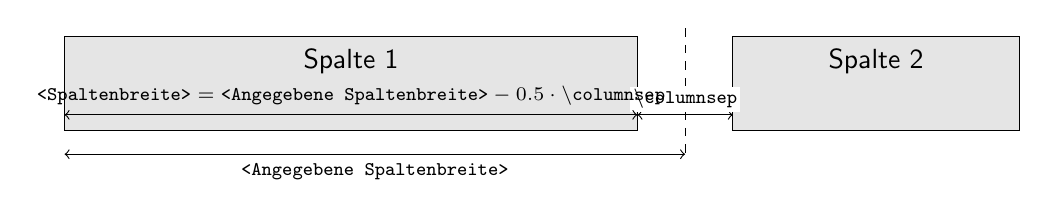
\begin{tikzpicture}[font=\scriptsize]
	\draw[fill=gray!20] (0,0) rectangle node[above, font=\sffamily] {Spalte 1} (0.6\textwidth, 1.2);
	\draw[fill=gray!20] (0.7\textwidth,0) rectangle node[above, font=\sffamily] {Spalte 2} (\textwidth, 1.2);

	\draw[dashed] (0.65\linewidth, 1.3) -- (0.65\linewidth, -0.35);

	\draw[<->] (0.6\linewidth, 0.2) -- node[above=1pt, fill=white, inner sep=1pt] {\texttt{\texttt{\textbackslash{}columnsep}}} (0.7\textwidth, 0.2);
	\draw[<->] (0, -0.3) -- node[below] {$\texttt{<Angegebene Spaltenbreite>}$} (0.65\textwidth, -0.3);
	\draw[<->] (0, 0.2) -- node[above] {$\texttt{<Spaltenbreite>} = \texttt{<Angegebene Spaltenbreite>} - 0.5 \cdot \texttt{\textbackslash{}columnsep}$} (0.6\textwidth, 0.2);
\end{tikzpicture}
\end{center}
}
%\[
%	\text{Tatsächliche linke Spaltenbreite} = \text{Angegebene linke Spaltenbreite} - 0.5 \cdot \text{Spaltenabstand}
%\]


\localeDE{
  \subsection{Grafikdateien einfügen}
  \label{sec:tut:grafik}
}

\localeDE{
In vielen Fällen möchte man neben einem Text eine passende Grafik einfügen.  Auch dies lässt sich einfach in \thepackage\ realisieren. Bevor wir uns diesem Anliegen widmen, noch einige grundlegende Aspekte zu Rastergrafiken in \thepackage:

Grafikdateien werden von \thepackage\ im Unterverzeichnis\footnote{Der Begriff \emph{Verzeichnis} wird in dieser Dokumentation synonym zu \emph{Ordner} verwendet.} \texttt{img} (engl. \emph{image} -- \emph{Bild}, \emph{Abbildung}) gesucht. Diese Maßnahme dient dazu, Ordnung im eigentlichen "`Arbeitsverzeichnis"' zu wahren. Das Einbinden von Grafiken geschieht grundsätzlich wie in \LaTeX\ üblich durch \Macro\includegraphics.

Die Umgebung \env{graphicscol} dient genau dem ursprünglich angesprochenen Zweck: Sie erzeugt zwei Spalten, wobei in der linken Spalte der Text und in der rechten Spalte die Grafik eingefügt wird. Die Verwendung von \env{graphicscol} soll anhand eines Beispiels erläutert werden. Als erstes Argument kann optional die Breite der linken Spalte angegeben werden (z.\,B. \SI{70}{\%} der Zeilenbreite, d.\,h. \texttt{0.7}\cs*{linewidth}). Es folgt die notwendige Angabe des Dateinamens (z.\,B. \texttt{image-example.jpg}). Abschließend können optional Optionen des Makros \cs*{includegraphics} angegeben werden, die auf die Grafik angewendet werden (z.\,B. \texttt{width=4cm}). Der Inhalt der Umgebung entspricht dem Text, der neben der Grafik angezeigt wird -- z.\,B. eine Aufgabe:
}

\startcode{de}
\begin{codefilecontent}{doc/tut-de-content-graphicscol}
\begin{graphicscol}[0.7\linewidth]{image-example.jpg}[width=4cm]
  Lorem ipsum dolor sit amet ...
\end{graphicscol}
\end{codefilecontent}
\endcode

\localeDE{
Um die Grafik links des Textes zu setzen, kann die Sternvariante \env{graphicscol*} genutzt werden, die ansonsten analog zu \env{graphicscol} verwendet wird.

Zusätzlich kann durch ein weiteres, optionales Argument bestimmt werden, wie die Grafik innerhalb ihrer Spalte horizontal ausgerichtet werden soll. Mögliche Angaben sind \texttt{l} für linksbündig, \texttt{r} für rechtsbündig und \texttt{c} für zentriert (engl. \emph{centered} -- \emph{zentriert}). Standardmäßig werden Grafiken in \env{graphicscol} rechtsbündig und in \env{graphicscol*} linksbündig ausgerichtet. Durch ein letztes optionales Argument kann spezifiziert werden, wie die Grafik innerhalb der Spalte vertikal ausgerichtet werden soll. Hierbei steht \texttt{t} für oben (engl. \emph{top} -- \emph{oben}, Standard) und \texttt{c} für zentriert.
}

\localeDE{
Verwandte Makros und Optionen:
\vspace{-0.25\baselineskip}
\begin{multicols}{3}\raggedcolumns
\begin{itemize}
	\item \opt{graphicspath}
\end{itemize}
\end{multicols}
}


\localeDE{\subsection{TikZ-Grafiken einfügen}}

\localeDE{
Grafiken können in \LaTeX\ auch mit dem Makropackage Ti\textit{k}z \cite{tikz} erstellt werden. Den Quellcode der Grafiken kann man dann in PGF-Dateien abspeichern und diese durch das Makro \cs{input} in sein Dokument einbinden. \thepackage\ erweitert das Einbinden von Ti\textit{k}z-Grafiken um einige Funktionen.

Wie bei Grafikdateien müssen die Grafiken in einem Unterverzeichnis des aktuellen Dokuments -- in diesem Fall mit dem Namen \texttt{tikz} -- vorliegen. An der jeweiligen Stelle des Dokument können die Grafiken dann durch \Macro\tikzinput eingebunden werden, z.\,B.
}

\startcode{de}
\begin{codefilecontent}{doc/tut-de-content-tikzinput-1}
\tikzinput{tikz-example.pgf}
\end{codefilecontent}
\endcode

\localeDE{
Da sich Grafiken zentriert meistens ansprechender ins Seitenlayout einfügen, existiert die Sternvariante \Macro{\tikzinput*}. Sie zentriert die Grafik zusätzlich mithilfe einer \env{center}-Umgebung:
}

\startcode{de}
\begin{codefilecontent}{doc/tut-de-content-tikzinput-2}
\tikzinput*{tikz-example.pgf}
\end{codefilecontent}
\endcode

\localeDE{
Überdies besteht die Möglichkeit, Ti\textit{k}z-Grafiken durch die \env{tikzcol}-Umgebung -- analog zu \env*{graphicscol} -- neben Text zu platzieren:
}

\startcode{de}
\begin{codefilecontent}{doc/tut-de-content-tikzcol}
\begin{tikzcol}[0.45\linewidth]{tikz-example.pgf}
  Lorem ipsum dolor sit amet ...
\end{tikzcol}
\end{codefilecontent}
\endcode

\localeDE{
Durch das erste, optionale Argument kann die Breite der linken Spalte angegeben werden, die den Text beinhaltet. Es folgt der notwendig anzugebende Dateiname, z.\,B. \texttt{tikz-example.pgf}. Bei der Sternvariante \env{tikzcol*} wird der Text rechts der Grafik gesetzt.

Ebenfalls verfügt \env{tikzcol} über zwei weitere Argumente, mit deren Hilfe die horizontale Ausrichtung durch \texttt{l} (links), \texttt{c} (zentriert) und \texttt{r} (rechts) bzw. die vertikale Ausrichtung durch \texttt{t} (oben) und \texttt{c} (zentriert) spezifiziert werden kann.
}

\localeDE{
Verwandte Makros und Optionen:
\vspace{-0.25\baselineskip}
\begin{multicols}{3}\raggedcolumns
\begin{itemize}
	\item \opt{tikzpath}
\end{itemize}
\end{multicols}
}


\localeDE{\subsection{Lösungen erstellen}}

\localeDE{
Häufig ist es hiflreich, auch Lösungen zu gestellen Aufgaben zu verfassen. 
Es gibt in \thepackage\ zwei Methoden, um dies zu  bewerkstelligen. Zum einen können Lösungen analog zu Aufgaben erstellt werden, was insbesondere bei längeren Lösungen (ausführliche Lösungen/Lösungswege/Musterlösungen) vorteilhaft ist. Hierzu existieren die Makros \Macro\sol\ (engl. \emph{solution} -- \emph{Lösung}) und \Macro\subsol als Pendants zu \cs{exe} und \cs{subexe}. Beide erwarten als notwendiges Argument den Titel der Lösung und verhalten sich auch sonst analog zu \cs{exe} und \cs{subexe}. Dies betrifft insbesondere die Nummerierung der Lösungs-Überschriften.
}

\startcode{de}
\begin{codefilecontent}{doc/tut-de-content-sol-subsol}
\sol{Loesung mit Unterloesungen}

\subsol{Erste Unterloesung}
Lorem ipsum dolor sit amet ...

\subsol{Zweite Unterloesung}
Lorem ipsum dolor sit amet ...
\end{codefilecontent}
\endcode

\localeDE{
Die Lösungen zu Teilaufgaben können auch im Zusammenhang von \Macro\sol und \Macro\subsol mithilfe der Umgebungen \env{mutliexelist} bzw. \env{multiexearray} und ihrer Varianten besetzt werden. Mit jedem Aufruf von \Macro\sol oder \Macro\subsol beginnt die Nummerierung der Teilaufgaben von vorne.

Die zweite Methode zum Erstellen von Lösungen verfolgt einen anderen Ansatz. Hierbei werden die Ergebnisse direkt nach den einzelnen Aufgaben oder Fragen eingefügt. Hierzu steht z.\,B. das Makro \Macro\res\ (engl. \emph{result} -- \emph{Ergebnis}) zur Verfügung. Als notwendiges Argument übergibt man ihm das Ergebnis der jeweiligen Aufgabe:
}

\startcode{de}
\begin{codefilecontent}{doc/tut-de-content-res-1}
\exe{Erste Aufgabe}

Lorem ipsum dolor sit amet ...

\res{Ergebnis der ersten Aufgabe}


\exe{Zweite Aufgabe}

Lorem ipsum dolor sit amet ...

\res{Ergebnis der zweiten Aufgabe}
\end{codefilecontent}
\endcode

\localeDE{
\thepackage\ ist so voreingestellt, dass diese Ergebnisse standardmäßig bei der Erzeugung des Arbeitsblattes nicht dargestellt werden. Um dies zu ändern, muss die Option \opt{showresults} verwendet werden:
}

\startcode{de}
\begin{codefilecontent*}{doc/tut-de-content-showresults}
\documentclass[showresults]{edu}
\end{codefilecontent*}
\endcode

\localeDE{
Es besteht die Möglichkeit, \Macro\res durch ein optionales Argument einen Alternativen Inhalt zu übergeben, der ausgegeben wird, wenn die Ergebnisse \emph{nicht} angezeigt werden sollen (d.\,h. im Standardfall bzw. bei \opt*{showresults=false}). Dies kann z.\,B. hilfreich sein, um einen manuellen Seitenumbruch oder einen zusätzlichen Abstand einzufügen, der in der Lösung nicht benötigt wird:
}

\startcode{de}
\begin{codefilecontent}{doc/tut-de-content-res-2}
\eduoption{showresults}{false}

Lorem ipsum dolor sit amet ...

\res[\vspace*{2cm}]{Ergebnis}

Lorem ipsum dolor sit amet ...
\end{codefilecontent}
\endcode

\localeDE{
Es kann hilfreich sein, auf erwartete Ergebnisse durch eine Linie oder eine Box hinzuweisen. Zu diesem Zweck können die Makros \Macro\resr\ (engl. \emph{rule} -- \emph{Linie}),  \Macro\resrfill\ und \Macro\resb\ (engl. \emph{box} -- \emph{Box}) verwendet werden. Diese verhalten sich grundsätzlich wie \cs{res}, zeigen die Ergebnisse also nur an, wenn \opt{showresults} gesetzt ist. Werden die Ergebnisse nicht angezeigt, erzeugen die ersten beiden jedoch eine vertikale Linie, letztes einen rechteckigen Rahmen.

Die Linie von \Macro\resr ist standardmäßig \SI{2}{cm} lang und befindet sich \SI{4}{pt} unterhalb der Grundlinie der Zeile. Durch zwei optionale Argumente können diese Eigenschaften manipuliert werden. Im folgenden Beispiel lautet das Ergebnis jeweils "`Sonett"', die Linie ist im zweiten Fall \SI{5}{cm} lang und befindet sich auf der Grundlinie (ist also um \SI{0}{cm} verschoben):
}

\startcode{de}
\begin{codefilecontent}{doc/tut-de-content-resr}
\eduoption{showresults}{false}

Lorem ipsum dolor sit amet: \resr{Sonett}

Lorem ipsum dolor sit amet: \resr[5cm]{Sonett}[0cm]
\end{codefilecontent}
\endcode

\localeDE{
Die Linie von \Macro\resrfill erstreckt sich bis zum Ende der aktuellen Zeile und befindet sich \SI{4}{pt} unterhalb der Grundlinie der Zeile, wobei sich dieser Versatz durch ein Optionales Argument verändern lässt. Hinter dem Makro sollte innerhalb einer Zeile kein Text mehr gesetzt werden, da es sonst du Darstellungsfehlern kommen kann.
Im folgenden Beispiel lautet das Ergebnis jeweils "`Loriot"', die Linie befindet sich im zweiten Fall auf der Grundlinie (ist also um \SI{0}{cm} verschoben):
}

\startcode{de}
\begin{codefilecontent}{doc/tut-de-content-resrfill}
\eduoption{showresults}{false}

Lorem ipsum dolor sit amet: \resrfill{Sonett}

Lorem ipsum dolor sit amet: \resrfill{Sonett}[0cm]

Lorem ipsum dolor sit amet.
\end{codefilecontent}
\endcode

\localeDE{
Die Box von \Macro\resb ist standardmäßig \SI{2}{cm} breit, \SI{0,65}{cm} hoch und um \SI{5}{pt} unter die Grundlinie verschoben. Auch diese Eigenschaften können durch optionale Argumente -- diesmal entsprechen drei Stück -- angepasst werden. Die Lösung der Folgenden Aufgabe lautet "`Wasserstoff"', die Box ist bei der zweiten Verwendung \SI{4}{cm} breit, \SI{1}{cm} hoch und um \SI{2}{pt} unter die Grundlinie verschoben:
}

\startcode{de}
\begin{codefilecontent}{doc/tut-de-content-resb}
\eduoption{showresults}{false}

Lorem ipsum dolor sit amet: \resb{Wasserstoff}

Lorem ipsum dolor sit amet: \resb[4cm][1cm]{Wasserstoff}[-2pt]
\end{codefilecontent}
\endcode

\localeDE{
Verwandte Makros und Optionen:
\vspace{-0.25\baselineskip}
\begin{multicols}{3}\raggedcolumns
\begin{itemize}
	\item \opt{solafterskip}
	\item \opt{solbeforeskip}
	\item \opt{solbg}
	\item \opt{solfg}
	\item \opt{sollabel}
	\item \opt{sollabelbg}
	\item \opt{sollabelfg}
	\item \opt{sollabelstyle}
	\item \opt{solnumberbg}
	\item \opt{solnumberfg}
	\item \opt{solnumberseparator}
	\item \opt{solnumberstyle}
	\item \opt{solstyle}
	\item \opt{subsolafterskip}
	\item \opt{subsolbeforeskip}
	\item \opt{subsolbg}
	\item \opt{subsolfg}
	\item \opt{subsollabel}
	\item \opt{subsollabelbg}
	\item \opt{subsollabelfg}
	\item \opt{subsollabelstyle}
	\item \opt{subsolnumberbg}
	\item \opt{subsolnumberfg}
	\item \opt{subsolnumberseparator}
	\item \opt{subsolnumberstyle}
	\item \opt{subsolstyle}
\end{itemize}
\end{multicols}
}


\localeDE{\subsection{Pseudo-A5-Druckvorlage und Folien}}

\localeDE{

\Warning{Mechanismus zum A5-Druck wird komplett überarbeitet.}

Es bietet es sich an, Dokumente mit wenig Inhalt in A5 anzufertigen. Der Druck auf A5 ist im heimischen Umfeld nicht immer unproblematisch. Auch das zweifache Drucken eines A5-Dokumentes auf ein A4-Blatt funktioniert nicht immer. Deshalb bietet sich häufig das folgende Prozedere an: Man druckt das Dokument in A4, skaliert es ansprechend auf irgendeinem Wege auf A5 und druckt es (meist im gleichen Schritt) zwei Mal auf ein A4-Blatt, welches abschließend in zwei A5-Blätter zerschnitten wird. Unabhängig davon, wie die nachträgliche Skalierung von A4 auf A5 vorgenommen wird, muss berücksichtigt werden, dass sich alle Elemente des Dokuments -- also insbesondere Schrift und Grafiken -- verkleinern. Auch Längen, die durch absolute Werte angegeben werden, sollten angepasst werden. 

\Todo{Teil zum A5-Druck fehlt.}

Möchte man Folien für Overhead-Projektoren erstellen, sollten einige Eigenschaften des Dokuments angepasst werden: Die Schrift muss (drastisch) vergrößert, Seitenränder hingegen können minimiert werden. Außerdem sollte serifenlose Schrift als Standardschrift verwendet werden, da sie die Lesbarkeit auf größerer Entfernung verbessert. Silbentrennung wird überdies deaktiviert. Durch die Option \opt{transparency} werden all diese Änderungen am Dokument durch \thepackage\ vorgenommen. Sie sollte beim Laden der Dokumentenklasse gewählt werden:
}

\startcode{de}
\begin{codefilecontent*}{doc/tut-de-content-transparency}
\documentclass[transparency]{edu}
\end{codefilecontent*}
\endcode


\localeDE{\subsection{Notizen}}

\localeDE{
Nachdem ein Arbeitsblatt verwendet oder eine Stunde abgehalten wurde, kann der Wunsch bestehen, Notizen auf betroffenen Dokumenten zu hinterlassen. So kann sich z.\,B. herausstellen, dass eine Aufgabe nicht verständlich gestellt war. Sollten resultierende Änderungen bei der Nachbereitung nicht direkt ins Dokument übernommen werden, können Sie als Notizen eingefügt werden. Standardmäßig werden Notizen durch Darstellung in farbiger serifenloser Schrift hervorgehoben und dargestellt. Einfache Textnotizen können durch das Makro \Macro\notet\ (engl. \emph{note} -- \emph{Notiz}) ergänzt werden:
}

\startcode{de}
\begin{codefilecontent}{doc/tut-de-content-notet}
\notet{2. Aufgabe: Aufgabenstellung nicht eindeutig.}
\end{codefilecontent}
\endcode

\localeDE{
Hat man in einem Arbeitsblatt Notizen ergänzt, möchte dieses jedoch noch einmal ohne diese Notizen erstellen, kann auf die Option \opt{shownotes} zurückgegriffen werden. Wird die Option nicht verändert, werden Notizen angezeigt. Unterdrückt werden Notizen durch den folgenden Aufruf:
}

\startcode{de}
\begin{codefilecontent*}{doc/tut-de-content-shownotes}
\documentclass[shownotes=false]{edu}
\end{codefilecontent*}
\endcode

\localeDE{
Insbesondere im Zusammenhang mit der Unterrichtsplanung (s.\,Abschnitt~\ref{sec:tut:unterrichtsplanung}) kann es hilfreich sein, horizontale Linien als Notizen einzufügen ("`Bis hier hin sind wir gekommen."'). Dies kann durch das Makro \Macro\notehr\ (engl. \emph{horizontal rule} -- \emph{horizontale Linie}) getätigt werden:
}

\startcode{de}
\begin{codefilecontent}{doc/tut-de-content-notehr}
Lorem ipsum dolor sit amet ...

\notehr

Lorem ipsum dolor sit amet ...
\end{codefilecontent}
\endcode

\localeDE{
Verwandte Makros und Optionen:
\vspace{-0.25\baselineskip}
\begin{multicols}{4}\raggedcolumns
\begin{itemize}
  \item \opt{notetstyle}
  \item \opt{notehrule}
  \item \opt{notetfg}
  \item \opt{notehrfg}
\end{itemize}
\end{multicols}
}



\localeDE{\section{Die erste Klassenarbeit}}

\localeDE{
Im zweiten Tutorial widmen wir uns dem Erstellen von Klassenarbeiten. Neben den grundlegenden Funktionen aus dem vorherigen Abschnitt~\ref{sec:tut:arbeitsblatt} verfügt \thepackage\ über Makros und Optionen zum Erstellen von Klassenarbeiten.

\Notice{Unter Verrechnungspunkten (VP) verstehen wir in diesem Abschnitt, die Punkte, man beim Lösen der einzelnen Aufgaben erhält und die abschließend in eine Note oder Notenpunkte (Sek~II) umgerechnet werden.}
}

\localeDE{\subsection{Zeile für Schülerdaten -- Viel Erfolg!}}

\localeDE{
Zuerst sollen die SchülerInnen ihren Namen auf die Klassenarbeit schreiben. Eine Vorlage stellt das Makro \Macro\makeexamtitle\ (engl. \emph{exam} -- \emph{Klausur, Prüfung}) zur Verfügung. Es erweitert den Titel von \cs{makeexamtitle} um drei Felder zum Ausfüllen: Als erstes können (bzw. sollen) die SchülerInnen eine ihnen eindeutig zugeordnete Nummer ergänzen, welche ihrer Stelle in der alphabetisch sortierten Klassenliste entspricht. Es bietet sich an, vor der ersten Klassenarbeit eine Folie mit der nummerierten Klassenliste anzufertigen und diese vor den Klassenarbeiten aufzulegen. Die Nummer vereinfacht das Sortieren der Klassenarbeiten vor der Korrektur. Des Weiteren sind Felder für Nach- und Vornamen vorhanden. Die Beschriftung und Länge der Felder kann durch Optionen beliebig angepasst werden. Neben den formalen Feldern wird zusätzlich eine kleine Mario-Figur am rechten Rand eingefügt, welche viel Erfolg wünscht.
}

\startcode{de}
\begin{codefilecontent}{doc/tut-de-content-makeexamtitle-1}
\makeexamtitle
\end{codefilecontent}
\endcode

\localeDE{
Das Makro verfügt über drei optionale Argumente. Mit dem ersten optionalen Argument kann der Text neben Mario verändet werden. Mit dem zweiten optionalen Argument kann man eine beliebige Grafikdatei spezifizieren, welche statt Mario eingesetzt wird. Hierbei müssen die Aspekte aus Abschnitt~\ref{sec:tut:grafik} berücksichtigt werden. Mithilfe des dritten und letzten optionalen Arguments kann die Höhe der selbst gewählten Graphik bestimmt werden. Standardmäßig ist diese \SI{2}{cm} hoch.

Im folgenden Beispiel wird die Graphik \texttt{image-example.jpg} in \SI{3}{cm} Höhe mit dem Text "`Viel Glück!"' verwendet:

\BugGit{72}
}

\startcode{de}
\begin{codefilecontent}{doc/tut-de-content-makeexamtitle-2}
\makeexamtitle[Viel Glueck!][image-example.jpg][3cm]
\end{codefilecontent}
\endcode

\localeDE{
  An dieser Stelle sei noch ein Mal auf das Makro \Macro\group verwiesen, mit desen Hilfe man zwei Verseionen der Klassenarbeit unterscheiden und jeweils einer Gruppe (z.\,B. Gruppe A und B) zuweisen kann. Die Bezeichnung der Gruppe wird im Titel neben der Grafik positioniert.
}

\localeDE{
Verwandte Makros und Optionen:
\vspace{-0.25\baselineskip}
\begin{multicols}{3}\raggedcolumns
\begin{itemize}
  \item \opt{examtitlefieldilabel}
  \item \opt{examtitlefieldiilabel}
  \item \opt{examtitlefieldiiilabel}
  \item \opt{examtitlefieldiwidth}
  \item \opt{examtitlefieldiiwidth}
  \item \opt{examtitlefieldiiiwidth}
  \item \opt{examtitlefieldsep}
  \item \opt{examtitlegraphicsheight}
  \item \opt{examtitlegraphicsscale}
\end{itemize}
\end{multicols}
}

\localeDE{
 \subsection{Verrechnungspunkte angeben}
 \label{sec:tut:vp}
}

\localeDE{
Bei Klassenarbeiten sollten die je Aufgabe erreichbaren VP aufgeführt werden. Zu diesem Zweck verfügen die aus Abschnitt~\ref{sec:tut:arbeitsblatt} bekannten Makros \Macro\exe und \Macro\subexe über optionale Argumente, durch welche diese VP angegeben werden können:
}

\startcode{de}
\begin{codefilecontent}{doc/tut-de-content-points-1}
\exe[5]{Erste Aufgabe}

Erste Aufgabe insgesamt 5VP

\subexe[2]{Erste Unteraufgabe}

Erste Unteraufgabe 2 VP

\subexe[3]{Zweite Unteraufgabe}

Erste Unteraufgabe 3 VP
\end{codefilecontent}
\endcode

\localeDE{
Sogar einzelnen Teilaufgaben (\env{multiexelist} oder \env{multiexearray}) können VP zugeteilt werden. Hierfür muss das Makro \Macro\points bedient werden. Normalerweise wird die Punktzahl hierbei direkt hinter den jeweiligen Inhalt der Teilaufgabe gesetzt, in der Sternvariante \Macro{\points*} wird sie hingegen an den rechten Rand der entsprechenden Zeile geschoben:
}

\startcode{de}
\begin{codefilecontent}{doc/tut-de-content-points-2}
\begin{multiexelist}
  \item Erste Teilaufgabe \points{1}
  \item Zweite Teilaufgabe \points*{2}
\end{multiexelist}

\begin{multiexearray}{2}
  Erste Teilaufgabe \points{3}  & Zweite Teilaufgabe \points{4} \\
  Dritte Teilaufgabe \points*{5} \\
\end{multiexearray}
\end{codefilecontent}
\endcode

\localeDE{
Werden in einer Klassenarbeit die in Abschnitt~\ref{sec:tut:fragen} vorgestellten Fragen verwendet, kann auch diesen jeweils durch ein optionales Argument eine Punktzahl zugeteilt werden:
}

\startcode{de}
\begin{codefilecontent}{doc/tut-de-content-points-3}
\exe[5]{Verstaendnisfragen mit insgesamt 5 VP}

\quest[2]{Erste Frage mit 2 VP}

\questblank

\quest[3]{Zweite Frage mit 3 VP}

\questtext{3}
\end{codefilecontent}
\endcode

\localeDE{
Durch die Optionen \opt{exepointsachieved} und \opt{subexepointsachieved} kann neben den VP der jeweiligen Aufgabe ein Feld für die erreichten VP eingefügt werden:
}

\startcode{de}
\begin{codefilecontent*}{doc/tut-de-content-exepointsachieved}
\documentclass[
  exepointsachieved,
  subexepointsachieved
]{edu}
\end{codefilecontent*}
\endcode



\localeDE{
Verwandte Makros und Optionen:
\vspace{-0.25\baselineskip}
\begin{multicols}{3}\raggedcolumns
\begin{itemize}
	\item \opt{exepointsachieved}
	\item \opt{exepointsachievedspace}
	\item \opt{exepointsachievedsep}
	\item \opt{exepointsfg}
	\item \opt{exepointslabel}
	\item \opt{exepointsleft}
	\item \opt{exepointsright}
	\item \opt{exepointsstyle}
	\item \opt{multiexepointsfg}
	\item \opt{multiexepointslabel}
	\item \opt{multiexepointsleft}
	\item \opt{multiexepointsright}
	\item \opt{multiexepointsstyle}
	\item \opt{questpointslabel}
	\item \opt{questpointsleft}
	\item \opt{questpointsright}
	\item \opt{questpointssep}
	\item \opt{questpointsstyle}
	\item \opt{subexepointsachieved}
	\item \opt{subexepointsachievedspace}
	\item \opt{subexepointsachievedsep}
	\item \opt{subexepointsfg}
	\item \opt{subexepointslabel}
	\item \opt{subexepointsleft}
	\item \opt{subexepointsright}
	\item \opt{subexepointsstyle}
\end{itemize}
\end{multicols}
}


\localeDE{\subsection{Bereiche für Ergebnisse}}

\localeDE{
\thepackage\ verfügt über die Möglichkeit, Bereiche zu erstellen, in denen die Ergebnisse der Klassenarbeit zusammengefasst werden können. Die kompakteste und einfachste Variante bildet das Makro \Macro\makeexamres\ (engl. \emph{result} -- \emph{Ergebnis}). Es erwartet als notwendiges Argument die Anzahl der maximal erreichbaren VP und erzeugt einen Kasten, in welchem die Anzahl der erreichten VP, die zugehörige Note, der Notendurchschnitt und der aktuelle Stand in der mündlichen Mitarbeit notiert werden kann. Des Weiteren ist ein Feld für die Unterschrift der/des Erziehungsberechtigten vorhanden. Durch Optionen kann der Kasten detailliert konfiguriert werden. So können z.\,B. die Felder für die mündliche Note oder die Unterschrift entfernt werden. Im folgenden Beispiel können 25\,VP erreicht werden:
}

\startcode{de}
\begin{codefilecontent}{doc/tut-de-content-makeexamres}
\makeexamres{25}
\end{codefilecontent}
\endcode

\localeDE{
Umfangreicher wird der Ergebnisbereich durch das Makro \Macro\makeexamrestable\ (engl. \emph{table} -- \emph{Tabelle}). Es erzeugt neben den aus \cs*{makeexamres} bekannten Feldern zusätzlich eine Tabelle, in der die je Aufgabe erreichten VP eingetragen werden können. Das Makro besitzt deshalb drei notwendige Argumente: Als erstes müssen die Nummern der Aufgaben (für gewöhnlich 1 bis $n$) angegeben werden. Anschließend die erreichbaren VP der jeweiligen Aufgaben (in gleichen Reihenfolge) und zum Schluss die Summe der insgesamt erreichbaren VP. Durch ein optionales Argument kann der SchülerInnenname ergänzt werden. Dies kann hilfreich sein, wenn die Ergebnisbereiche gesondert gedruckt werden sollen. Im folgenden Beispiel liegen die Aufgaben 1 bis 7 vor, für die 2, 4, 6, \dots, 14\,VP vergeben und somit ingsgesamt 56\,VP erreicht werden können. Der Ergebnisbereich soll für Horst Schlämmer personalisiert werden.
}

\startcode{de}
\begin{codefilecontent}{doc/tut-de-content-makeexamrestable}
\makeexamrestable[Horst Schlaemmer]{1, 2, 3, 4, 5, 6, 7}{2, 4, 6, 8, 10, 12, 14}{56}
\end{codefilecontent}
\endcode

\localeDE{
\Notice{Die durch \Macro\makeexamrestable erstellte Tabelle bietet Platz für maximal 10 Aufgaben.}
}

\localeDE{
Verwandte Makros und Optionen:
\vspace{-0.25\baselineskip}
\begin{multicols}{3}\raggedcolumns
\begin{itemize}
  \item \opt{exampointsaveragelabel}
  \item \opt{exampointsmarklabel}
  \item \opt{exampointsoflabel}
  \item \opt{exampointssecondmark}
  \item \opt{exampointssecondmarklabel}
  \item \opt{exampointssignature}
  \item \opt{exampointssignaturelabel}
  \item \opt{exampointstableexelabel}
  \item \opt{exampointstablelabel}
  \item \opt{exampointstablemaxlabel}
  \item \opt{exampointstablesumlabel}
  \item \opt{exampointstabletype}
  \item \opt{exampointstablewidth}
\end{itemize}
\end{multicols}
}

\localeDE{
  \section{Die erste Unterrichtsplanung}
  \label{sec:tut:unterrichtsplanung}
}



\localeDE{\section{Erscheinungsbild anpassen}}

\localeDE{\subsection{Fußzeile}}
